\documentclass{standalone}
\usepackage{tikz}
\usepackage{ctex,siunitx}
\usepackage{tkz-euclide}
\usepackage{amsmath,mathabx}
\usetikzlibrary{patterns, calc}
\usetikzlibrary {decorations.pathmorphing, decorations.pathreplacing, decorations.shapes,}
\begin{document}
\small
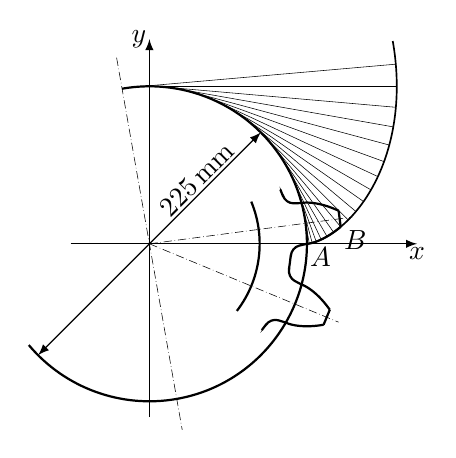
\begin{tikzpicture}[>=latex,scale=2.0,inner sep=1pt]
  \draw[->](-0.5,0)--(1.7,0)node[below]{$x$};
  \draw[->](0,-1.1)--(0,1.3)node[left]{$y$};
  \draw[very thin,densely dashdotted](100:1.2)--(100:-1.2);
  \draw[thick](100:1.0)arc(100:-140:1.0);
  \draw[<->](-135:1.0)--(45:1.0)node[sloped,pos=0.75,above]{$\diameter\qty{225}{mm}$};
  \draw[thick](22.5:0.7)arc(22.5:-37.5:0.7);
  \foreach \x in {7.5,-22.5}
  {
    \draw[very thin,densely dashdotted](0,0)--(\x:1.3);
    \draw[thick,rounded corners=3pt](\x+7.5:1.0)--(\x+9:0.9)arc(\x+9:\x+15:0.9);
    \draw[thick,rounded corners=3pt](\x-7.5:1.0)--(\x-9:0.9)arc(\x-9:\x-15:0.9);
  }
  \draw[thick,rotate=0,domain=0:40,samples=200] plot ({1.0*(cos(\x)+\x/180*pi*sin(\x))},{1.0*(sin(\x)-\x/180*pi*cos(\x))})coordinate(M');
  \draw[thick,rotate=15,domain=0:40,samples=200] plot ({1.0*(cos(\x)+\x/180*pi*sin(\x))},{-1.0*(sin(\x)-\x/180*pi*cos(\x))})coordinate(N');
  \draw[thick](M')--(N');
  \draw[thick,rotate=-30,domain=0:40,samples=200] plot ({1.0*(cos(\x)+\x/180*pi*sin(\x))},{1.0*(sin(\x)-\x/180*pi*cos(\x))})coordinate(M);
  \draw[thick,rotate=-15,domain=0:40,samples=200] plot ({1.0*(cos(\x)+\x/180*pi*sin(\x))},{-1.0*(sin(\x)-\x/180*pi*cos(\x))})coordinate(N);
  \draw[thick](M)--(N);
  % \begin{scope}[rotate=82.5]
  \draw[semithick,domain=0:100,samples=200] plot ({1.0*(cos(\x)+\x/180*pi*sin(\x))},{1.0*(sin(\x)-\x/180*pi*cos(\x))});
  \foreach \x in {0,5,...,95}
  {
    \draw[very thin](\x:1)--({1.0*(cos(\x)+\x/180*pi*sin(\x))},{1.0*(sin(\x)-\x/180*pi*cos(\x))});
    % \draw[very thin](\x:1)--(\x:0.6);
  }
  \node at (0:1)[below right]{$A$};
  \node at ({1.0*(cos(40)+40/180*pi*sin(40))},{1.0*(sin(40)-40/180*pi*cos(40))})[below right]{$B$};
  % \end{scope}
  % \draw(0.8,1.42)--++(135:0.2)--++(0.5,0)node[above left]{渐开线};
\end{tikzpicture}
\end{document}